\chapter{DSDV}
\label{chap:dsdv}

\section{Ejercicio 2.1}

\subsection{Avanza la simulación hasta el instante t = 7 s. Busca el primer paquete Hello transmitido a partir a ese
instante con un valor de hopdistance de al menos 3 y muestra una captura del contenido. Explica el significado
de los campos srcAddress y nextAddress, utilizando para explicarlos una captura de la tabla de enrutamiento del
nodo que está transmitiendo el paquete (i.e., no el que consta en srcAddress)}

\begin{figure}[H]
    \centering
    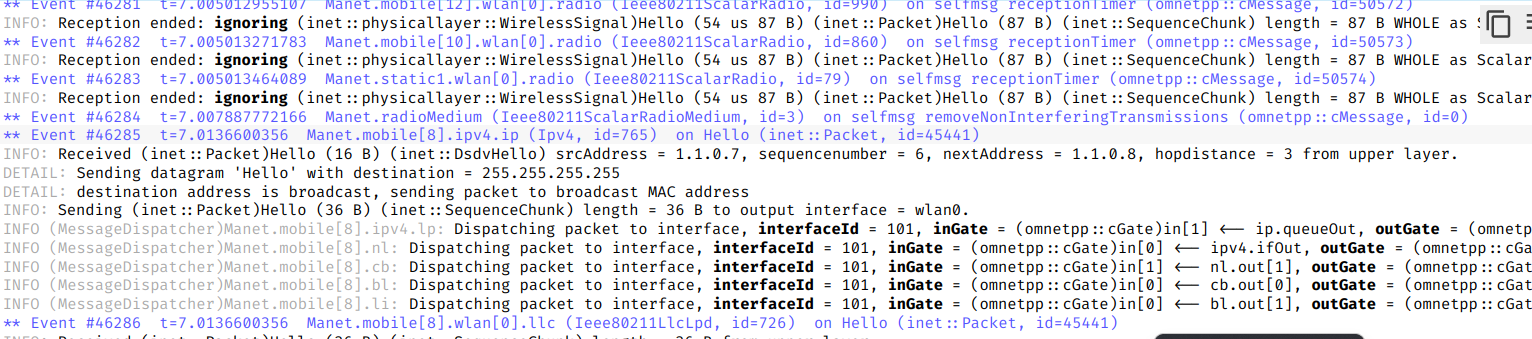
\includegraphics[width=155mm, scale=0.75]{imaxes/dsdv/ejercicio2_1.png}
    \caption{Log del nodo que manda el primer Hello con hopdistance 3}
    \label{fig:ejer2_1}
\end{figure}

Como se puede ver la imagen, el nodo que manda el primer mensaje Hello con hopdistance 1 es el nodo 8. Vamos a fijarnos en su tabla de enrutamiento:

\begin{figure}[H]
    \centering
    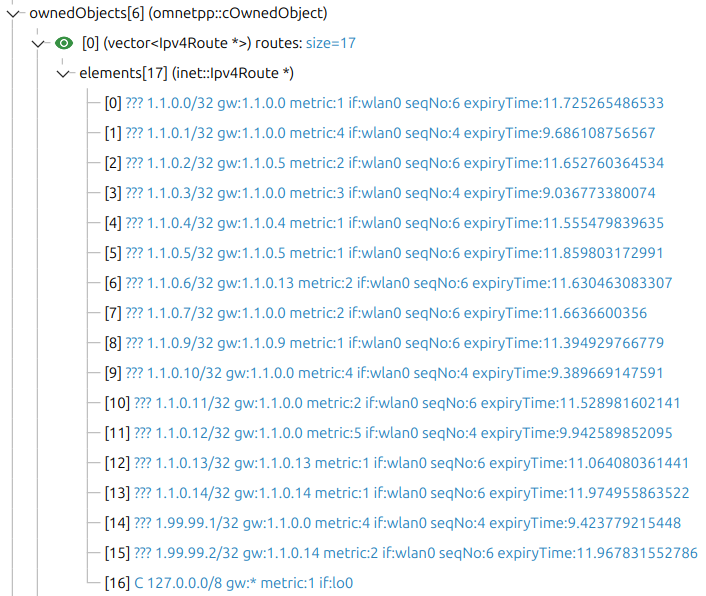
\includegraphics[width=115mm, scale=0.75]{imaxes/dsdv/ejercicio2_1_2.png}
    \caption{Tabla de enrutamiento nodo 8}
    \label{fig:ejer2_1}
\end{figure}

Según la imagen \ref{fig:ejer2_1}, el campo srcAddress es el nodo que envía el paquete Hello, en este caso es el 1.1.0.7 y el campo nextAddress es la siguiente dirección que va a recibir la trama, en este caso 1.1.0.8. 



\section{Ejercicio 2.2}

\subsection{¿Qué valor tiene de sequencenumber? ¿Qué quiere decir ese valor?}

\section{Ejercicio 2.3}

\subsection{¿Cómo se modifica? ¿Qué nodo lo modifica, y cuándo lo hace?}

\section{Ejercicio 2.4}

\subsection{Muestra la tabla de enrutamiento del nodo que recibe el Hello de la pregunta anterior justo antes y justo
después de recibirlo, relacionándola con el contenido del paquete. Si se actualiza la tabla, explica por qué se
actualiza y las entradas que se crean. Si no se actualiza, explica por qué no se actualiza y di qué entrada se
crearía (destino, gateway, métrica) si se actualizase con la información del paquete.}

\section{Ejercicio 2.5}

\subsection{Avanza hasta la caída del nodo en t = 15 s. Ten en cuenta que la ruta en ese momento puede ser diferente a
la de AODV, y por lo tanto el nodo a desactivar también. ¿Cuál es el primer nodo en darse cuenta de la caída?
¿Notifica la caída del nodo de alguna forma?}

\section{Ejercicio 2.6}

\subsection{¿Cómo se repara la ruta entre static1 y static2? ¿En qué momento?}

